\section*{Abstract}
% ============================================================

%%> [TODO — Jessica Elisma]
%%> The abstract has not been submitted. Per the guiding structure,
%%> it should be a single paragraph (max 300 words) covering:
%%>   1. Title and authors (already handled by \maketitle above)
%%>   2. Background and knowledge gap
%%>   3. Study aim and justification
%%>   4. Methodology summary (quantitative and qualitative)
%%>   5. Main results and findings
%%>   6. Interpretation and conclusions
%%> Abstracts do not contain citations.
%%>
%%> CONCEPTUAL NOTE: The abstract should frame the core comparison
%%> clearly: supercooling (brine bath, liquid state maintained)
%%> versus flash freezing (acetone-dry ice, solidification induced).
%%> The central argument is that supercooling avoids the freeze-thaw
%%> cycle entirely, which is the primary source of cellular damage
%%> in the flash-frozen group. Make sure this distinction is explicit.

Freezing is a well-established food preservation method. However, 
the ice crystals created in foods through freezing can damage them, 
limiting their usable life. Supercooling involves reducing a food’s 
temperature beyond its fluids’ freezing point, thus possibly limiting 
damage to the food’s structure. This experiment determined whether 
supercooling methods prevent damage that would otherwise occur to foods, 
specifically fruits, during freezing. The two methods of preservation 
were compared experimentally. Freezing was attained by placing grape 
and apple samples in an acetone and dry-ice bath and samples were placed 
in an ice and brine solution for supercooling. Samples were massed prior 
to and following freezing and supercooling and temperature was monitored 
throughout the procedure. Microstructure analysis was also conducted 
before and after the procedure. Mass losses were observed in all groups, 
although the freeze-thaw cycle caused greater losses in the acetone-dry 
ice group. Qualitatively, the fruits’ physical properties were better 
conserved after supercooling. These results concur with our hypothesis 
and confirm that supercooling causes less damage to foods than freezing.

% ============================================================
\section{Objective}
% ============================================================

\contributor{Erqi Wei}

The aim of this experiment was to compare supercooling in an ice-water
brine bath and flash freezing in a dry ice-acetone bath for the short
term preservation of apples and grapes. Apples and grapes were used as
two fruit types that differ in water content and tissue integrity, and
the physical properties examined were mass loss, texture, and
microscopic structure.

The working hypothesis was that supercooling would preserve the fruit's
physical properties better than flash freezing because it avoids the
freeze-thaw cycle.

% ============================================================
\section{Methodology}
% ============================================================

\contributor{Victor Zhan, Ahjin Joo, Savva Zosimov}

The sample fruits of the experiment consisted of store-bought seedless
green grapes and Red Prince apples, which have freezing points of around
$-$2.2~°C and $-$1.7~°C respectively \cite{zhao2025, wflo2018}. The
fruits were cut into small rectangular prisms of roughly 2.5~$\times$~1.0~$\times$~0.5~cm
beforehand to speed up the cooling process. The experiment was divided into two parts: supercooling of apples and grapes in an ice-water brine bath and flash-freezing of the same fruits in a dry ice--acetone bath. For the brine bath, 100~mL of water was placed into a container and 50~g of NaCl was added, as well as a magnetic stir bar to maintain uniform cooling throughout the bath. Ice was introduced in 50~g increments until the mixture reached $-$8~°C. The fruit samples were placed in plastic bags, excess air was removed, and the samples were submerged in the cooling bath and left undisturbed for 15--20~min. The temperature was monitored, and the minimum supercooled temperature reached by each sample was recorded when the fruit remained unfrozen below 0~°C. For the rapid freezing method, a dry ice--acetone bath was prepared inside a fume hood: dry ice was placed into a Styrofoam container and a large beaker was placed within it. Approximately 5~L of acetone was poured into the beaker, and the mixture was allowed to cool to about $-$30~°C. Fruit samples were placed in dry test tubes and fully submerged in the bath. Using an infrared thermometer, sample temperatures were monitored continuously and the temperature at which solidification began was recorded. After treatment, final masses were measured, mass loss was calculated, and post-treatment characteristics were recorded. The flash-frozen samples were then allowed to thaw at room temperature before the same measurements were repeated. For microscopic analysis, fresh fruit samples that had not undergone freezing were sliced into approximately 0.5~mm slivers using a razor blade. Each sliver was placed on a glass microscope slide and positioned on the microscope stage. Magnification was increased incrementally, and images were taken at magnifications of 4$\times$, 10$\times$, and 40$\times$. The same procedure was repeated for the supercooled samples and the thawed flash-frozen samples.

% ============================================================
\section{Results}
% ============================================================

\contributor{Justin Zheng, Taslima Nahar, Alex Hanwen Qiu, Sarah Ann Carey, Micheal Murai, Logan Joffre}

\begin{table*}[t]
\centering
\caption{Average Recorded Temperature by Method and Fruit}
\label{tab:temp}
\begin{tabular}{llccc}
\toprule
Method & Fruit & Average Temp. (°C) & Median Temp. (°C) & Std. Dev. (°C) \\
\midrule
Ice-Water Bath   & Grape & $-$3.29  & $-$3.50  & 2.12 \\
Ice-Water Bath   & Apple & $-$2.79  & $-$3.10  & 1.5  \\
Acetone-Dry Ice  & Grape & $-$15.03 & $-$15.00 & 4.88 \\
Acetone-Dry Ice  & Apple & $-$13.30 & $-$14.00 & 2.82 \\
\bottomrule
\end{tabular}
\end{table*}

\begin{table*}[t]
\centering
\caption{Average Mass Loss by Method and Fruit}
\label{tab:mass}
\begin{tabular}{llccc}
\toprule
Method & Fruit & Avg. Mass Loss (g) & Median Mass Loss (g) & Std. Dev. (g) \\
\midrule
Ice-Water Bath   & Grape & 0.0462 & 0.0436 & 0.0345 \\
Ice-Water Bath   & Apple & 0.0269 & 0.0280 & 0.0184 \\
Acetone-Dry Ice  & Grape & 0.0458 & 0.0345 & 0.0284 \\
Acetone-Dry Ice  & Apple & 0.0416 & 0.0227 & 0.0427 \\
\bottomrule
\end{tabular}
\end{table*}

\begin{figure}[h]
\centering
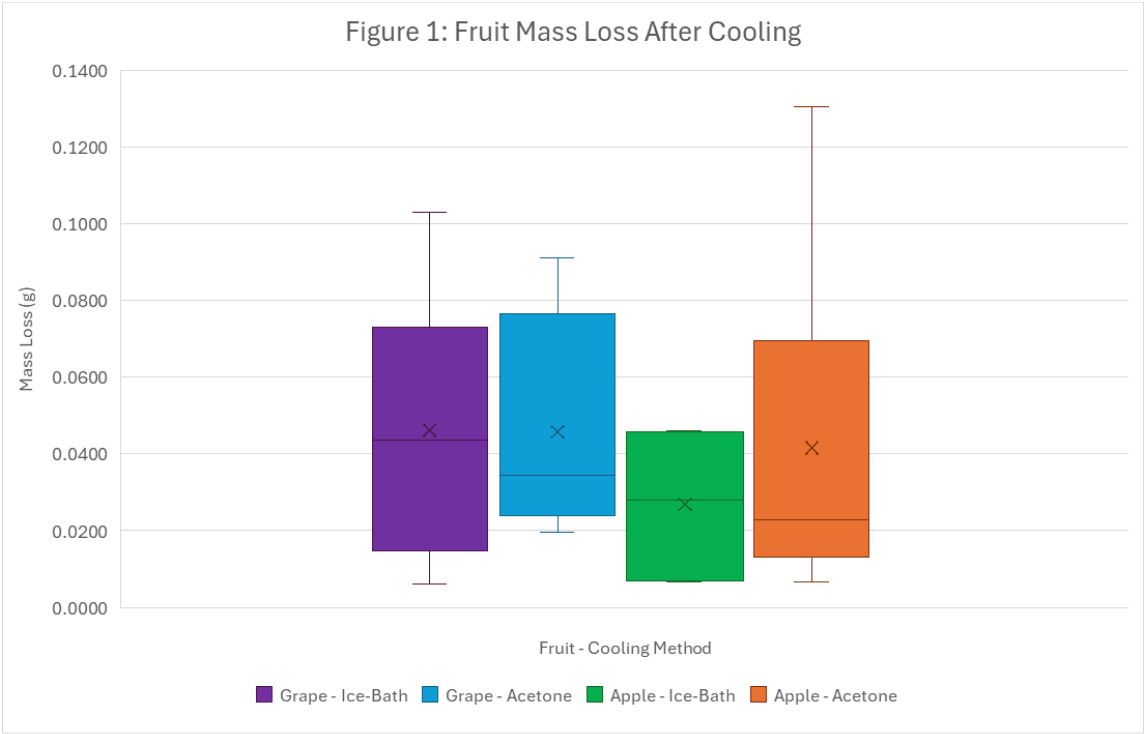
\includegraphics[width=0.45\linewidth]{media/image1.png}
\caption{Mass loss by fruit and cooling method.}
\label{fig:massloss}
\end{figure}

\begin{figure}[h]
\centering
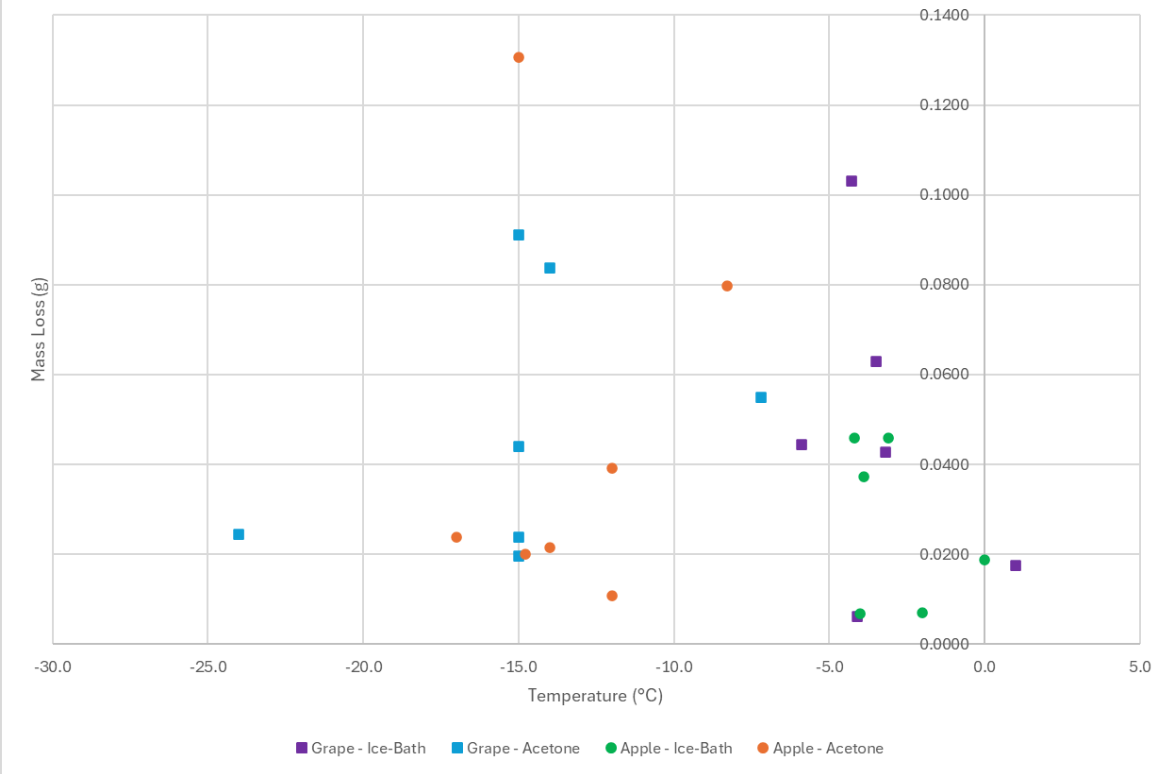
\includegraphics[width=0.45\linewidth]{media/image2.png}
\caption{Mass loss relative to recorded temperature.}
\label{fig:massvstemp}
\end{figure}

\textbf{Texture}

The supercooled grapes were initially flexible, gelatinous and
translucent. After treatment, they became more fragile and less
structured. The supercooled apples were initially fibrous, 
opaque and rigid, and after treatment they became softer,
soggier and more translucent.

The flash-frozen grapes started with similar initial descriptors, but
after thawing they were more fragile and mushy.
The flash-frozen apples changed from fibrous, opaque and rigid to be more
flexible, smooth and soft.

These observations were qualitative, since we did not have a texture
analyzer.

\begin{figure}[h]
\centering
\begin{minipage}[t]{0.3\linewidth}
\centering
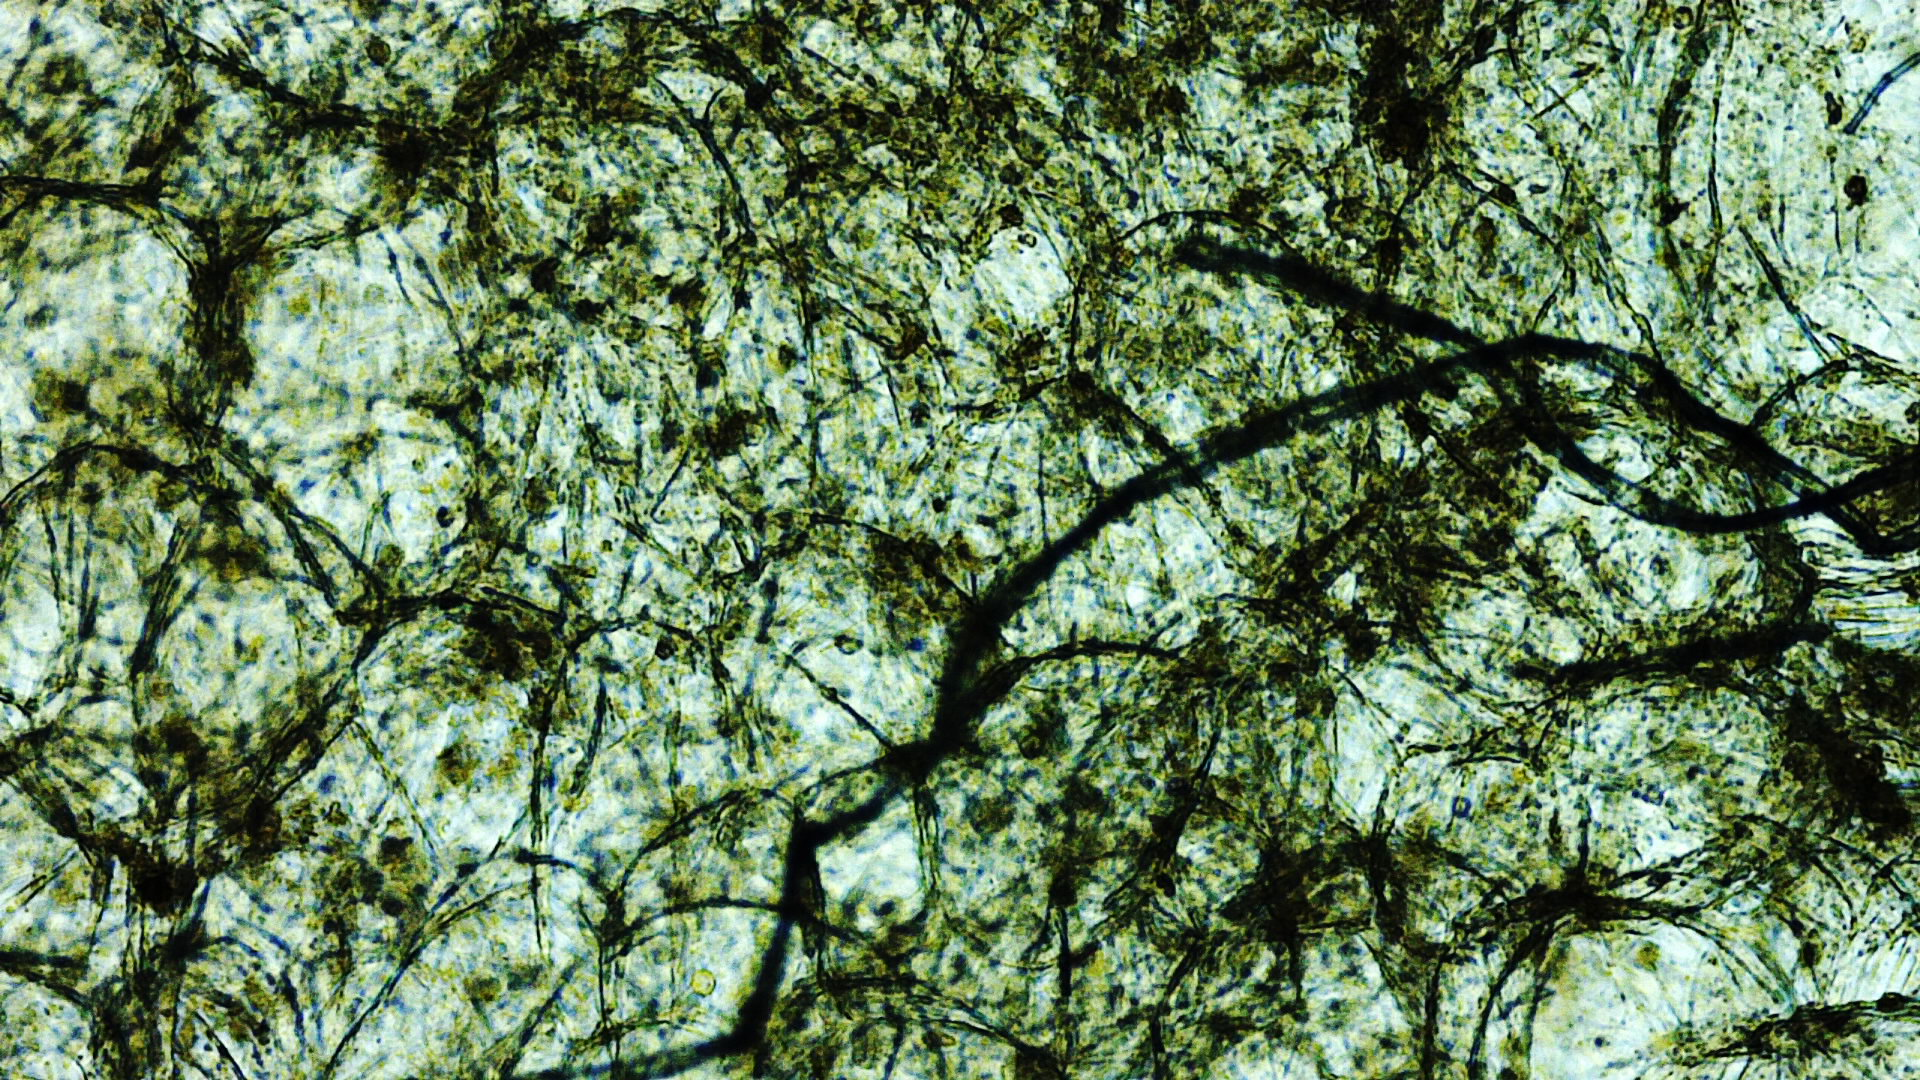
\includegraphics[width=\linewidth]{media/4X_I_GRAPE1.JPG}
\par\small Initial (I)
\end{minipage}\hfill
\begin{minipage}[t]{0.3\linewidth}
\centering
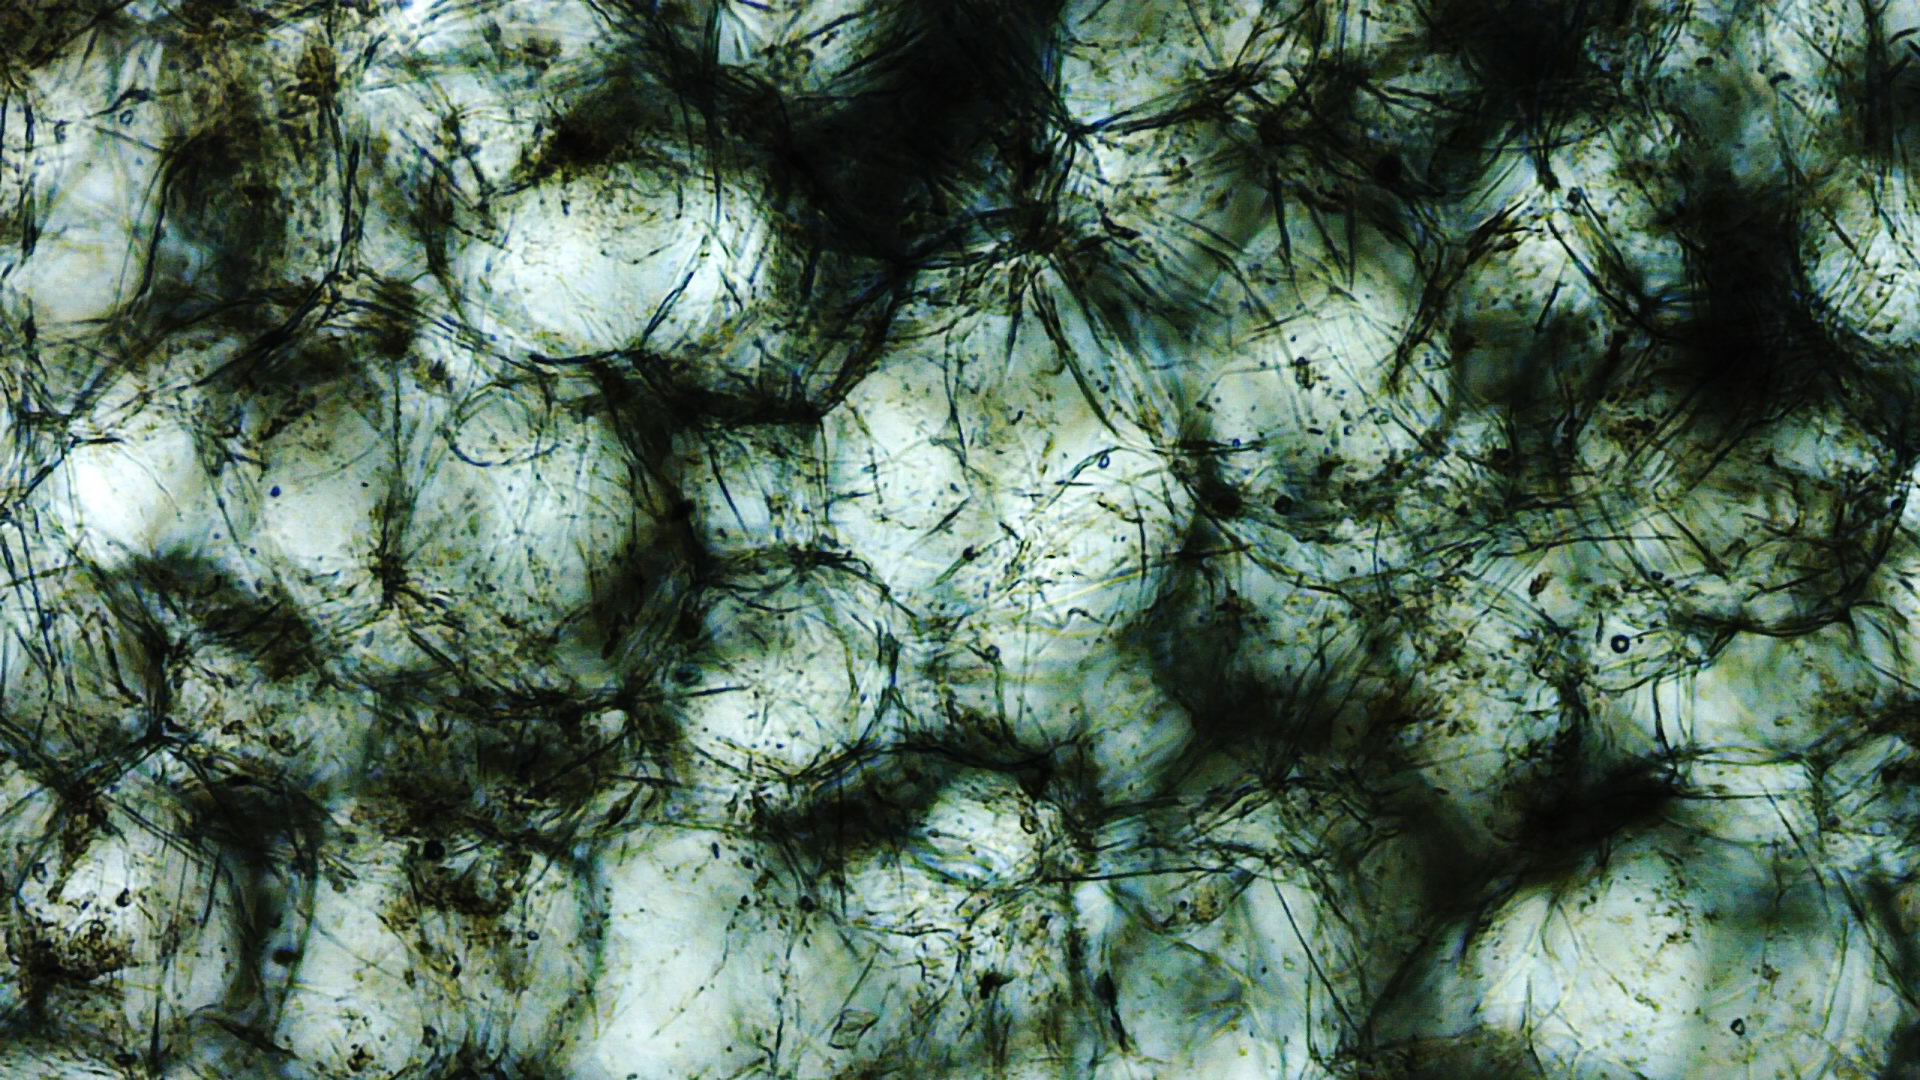
\includegraphics[width=\linewidth]{media/4X_F_GRAPE1.JPG}
\par\small Frozen (F)
\end{minipage}\hfill
\begin{minipage}[t]{0.3\linewidth}
\centering
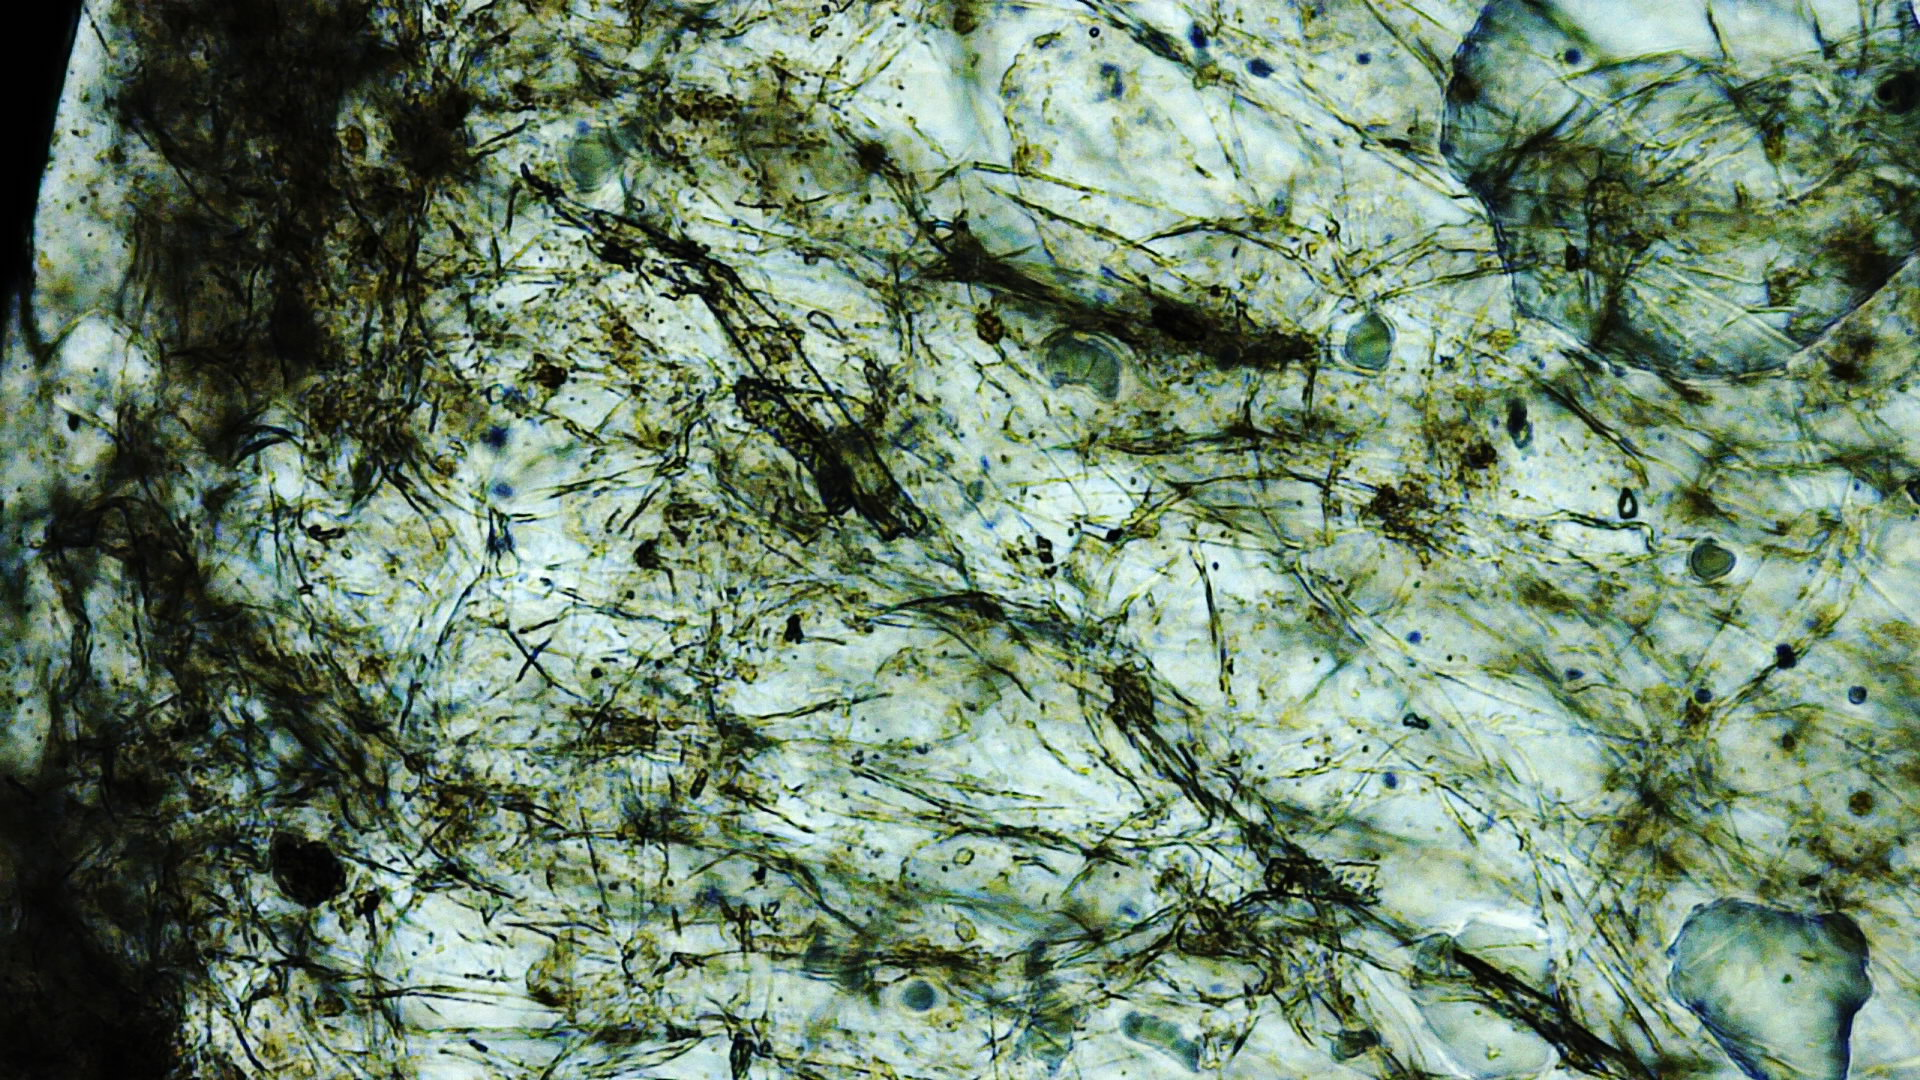
\includegraphics[width=\linewidth]{media/4X_S_GRAPE1.JPG}
\par\small Supercooled (S)
\end{minipage}
\caption{40x grape microscope images: initial (I), frozen (F), and
supercooled (S).}
\label{fig:grape40x}
\end{figure}

The results demonstrate that cooling rate significantly affected the
fruit samples, but faster cooling did not consistently result in better
preservation after thawing. The acetone--dry ice bath reached much lower
temperatures (as low as $-$30~°C) compared to the ice-water bath, which
remained closer to $-$2 to $-$6~°C. Table \ref{tab:temp} and Figure
\ref{fig:massvstemp} show that the lower temperatures did not
consistently produce smaller mass losses.

Mass measurements in Table \ref{tab:mass} and Figure \ref{fig:massloss}
show that grapes generally experienced greater mass loss compared to apples. The apples had more significant mass loss in the acetone--dry 
ice bath than in the ice-water bath, explained by ice crystals disrupting cell membranes and releasing water during thawing. For the brine group, mass loss was not from thawing drip because the fruit remained supercooled rather than frozen.

Microscopic observations in Figure \ref{fig:grape40x} showed evidence of structural disruption in thawed samples, which displayed deformed and less organized cell structures compared to initial samples.

Figure \ref{fig:grape40x} shows the 40x grape micrographs for the initial (I), frozen (F), and supercooled (S) samples. Microstructure analysis shows that flash freezing using acetone and a dry ice bath causes more damage to cell structure than supercooling by ice-water and brine. In microscopic images of both supercooled and frozen grape samples, there is a loss of fibers, indicating structural damage. However, the frozen grapes showed more fiber loss and also had dark regions, which could indicate damage to cell tissue. Additionally, the 10x image of the supercooled grape sample shows a large amount of fibers, which can be seen by the large amount of lines present in the picture. As such, the structural integrity of the sample is mostly maintained. For the apple samples, flash freezing causes ice formation which results in cell structure damage. The frozen samples showed bubbles forming within the dark regions which are indicative of ice crystal formation. The solidification of water to ice causes expansion, which creates air pockets.

The literature says that faster freezing causes less cell damage due to
the distribution of the ice crystals being distributed evenly.
Flash freezing thus has a lesser effect on the cell structures and
textures of the fruits than slow cooling \cite{narayana2023}. However,
our observations do not back this up very well.

There was a difference in texture from before and after supercooling
consistent with water loss and structure denaturation. There was a lack
of consistency between the texture results. Since we did not have an
accurate way of measuring texture and thus used subjective descriptions,
it may not be possible to accurately use this data. Mostly, the fruits
became more malleable, supposedly from structures being broken by the
freezing temperatures and the expansion of the water in the cells. There
were instances when the grape, which seems more affected by the
supercooling process, was reduced to a pulpy substance, practically
devoid of structure. Comparing this to the significant decrease in the
	lines observed in Figure \ref{fig:grape40x}, it can be deduced that the
diminished presence of stabilizing cell components is causing the
decreased structural integrity of the grape. The apple seemed to
experience less significant structural changes and sometimes became
firmer than it was previously, though it generally became more malleable
as well.

Additionally, flash-freezing with the acetone-dry ice bath was faster
and the temperatures could reach $-$30~degrees Celsius, compared to
approximately $-$3~degrees in the ice-bath experiments, which should have
preserved the fruits better, according to previous literature, but we
observed that the acetone-dry ice bath had a more damaging effect on the
fruits, perhaps because of the short amount of time that the fruits were
kept submerged \cite{narayana2023}.

The freezing process in the acetone group likely caused the fruit
samples to lose mass because ice crystals formed and punctured the cell
membranes, allowing water and other substances to leak out during
thawing \cite{lorv2014}. That explanation applies to the flash-frozen
samples, but it does not directly explain the brine group, which did
not undergo a freeze-thaw cycle.

Drip loss from freeze-thaw cycles explains the greater mass loss in grapes compared to apples, as shown in Table \ref{tab:mass} and Figure \ref{fig:massloss}.


There was a general tendency for grapes to lose more mass than apples.
The cell structure changes were also different between the fruits: grapes were
initially more watery and ended up more fragile, while apples started
firmer and softened after treatment. This supports the idea that fruit
type mattered as much as cooling temperature.

% ============================================================
\section{Conclusion}
% ============================================================

\contributor{Nicole Zhang}

The aim of this experiment was to compare supercooling in an ice-water
brine bath with flash-freezing in a dry-acetone solution. The objective
was achieved as the effects of both cooling methods on the fruits were
successfully observed. Our hypothesis was confirmed, as supercooling 
retained more of the fruits' physical properties than flash freezing, which
caused more damage due to the freeze-thaw cycle. The results suggest that
supercooling is a more effective method for preserving the texture and
structure of fruits compared to flash freezing. To
improve this experiment, a wider variety of fruits could be tested to
compare how different cellular structures respond to cooling.
Additionally, future studies could examine long-term preservation using
both methods, as well as changes in taste and nutrient content.
